\section{Network Results}
\subsection{Method of reflection}

We conducted an in-depth analysis of the Symptom Influence (\textit{SI}) and Disease Influence (\textit{DI}) indices,
considering both level-1 and level-2 metrics in our symptom-disease network.

\subsubsection*{Level-1 Metrics}


For the level-1 metrics, which quantify the individual prevalence of symptoms and diseases,
we observed distinctive patterns, as illustrated in Figure~\ref{fig:DegreeDistribution}.
The Symptom Influence (\textit{SI}) at level-1, representing the number of diseases associated with a symptom, demonstrated a wide distribution,
ranging predominantly between 0 and 60. This suggests that certain symptoms exhibit a broad association with various diseases,
showcasing the diverse nature of symptom-disease relationships.\\
Conversely, the Disease Influence (\textit{DI}) at level-1, reflecting the number of symptoms related to a disease,
exhibited a narrower range, typically falling between 2 and 12.
This narrower range indicates that diseases tend to have a more focused set of associated symptoms.
\begin{figure}[H]
    \centering
    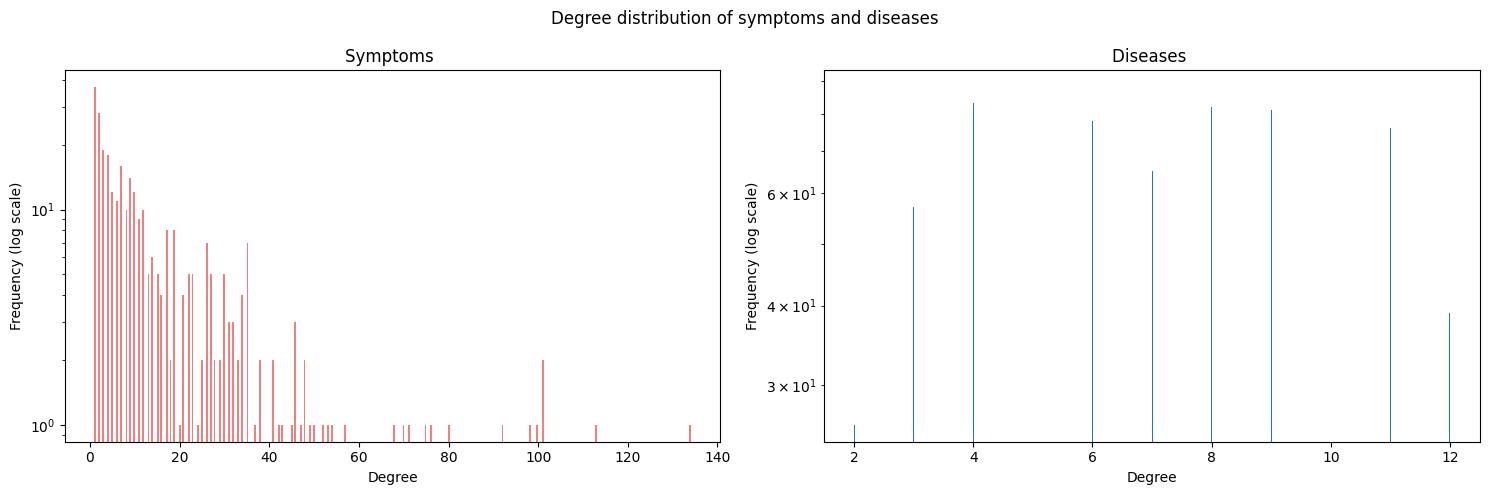
\includegraphics[width=\columnwidth]{degree_distribution.png}
    \caption{Degree Distribution (level 1)}
    \label{fig:DegreeDistribution}
\end{figure}

\subsubsection*{Level-2 Metrics}
Moving to the level-2 metrics, which capture the interconnectedness and broader impact of symptoms or diseases within the network,
we uncovered intriguing patterns (see Figure~\ref{fig:l2_distribution}).
The Symptom Influence (\textit{SI}) at level-2, reflecting the presence of symptoms across diseases and their associations with other symptoms,
exhibited values ranging from 4 to 12.
This suggests that certain symptoms not only co-occur within diseases but also form meaningful connections with a diverse set of other symptoms.
A higher level-2 Symptom Influence (\textit{SI}) implies a symptom's propensity to be associated with a wide range of symptoms,
indicating its potential impact on various disease pathways.\\
On the other hand, the Disease Influence (\textit{DI}) at level-2, quantifying the ripple effects of a disease's symptoms on other diseases,
demonstrated a wider range, typically spanning from 10 to 80.
This broader range signifies that certain diseases have a more extensive influence on the network by affecting a multitude of other diseases.
A higher level-2 Disease Influence (\textit{DI}) implies that a disease's symptoms not only contribute to its immediate associations
but also have far-reaching consequences, affecting a network of interconnected diseases.\\
These results highlight the diverse roles played by symptoms and diseases in influencing the network when considering higher-order interactions.


\begin{figure}[H]
    \centering
    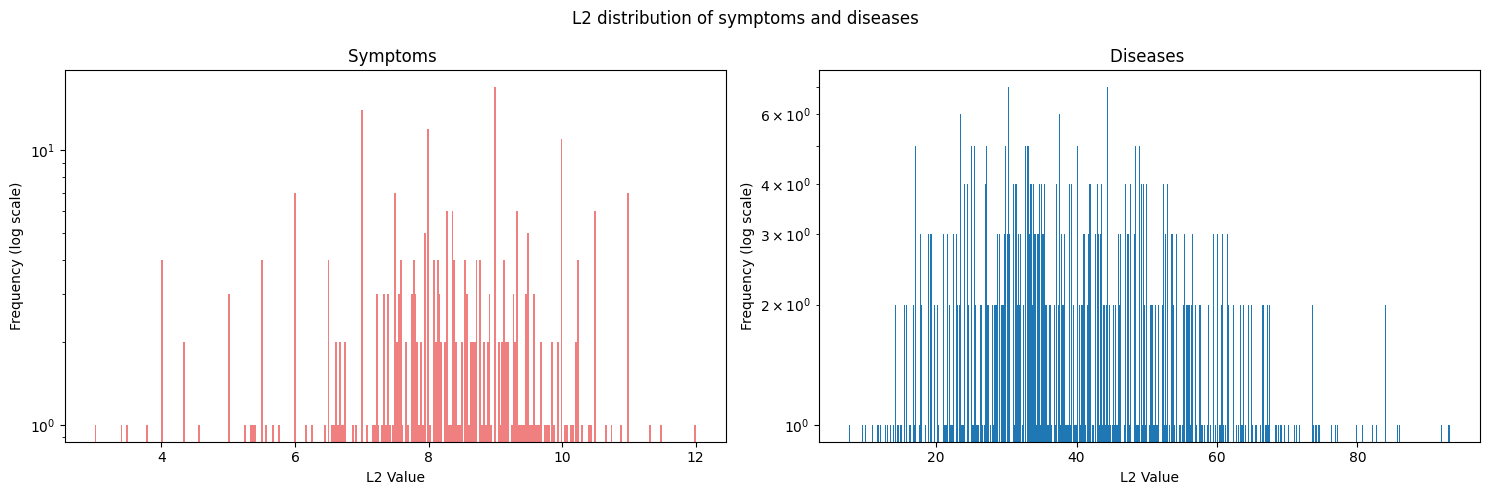
\includegraphics[width=\columnwidth]{L2_distribution.png}
    \caption{L2 Distribution for both symptoms and diseases}
    \label{fig:l2_distribution}
\end{figure}
\subsubsection*{Power Law CCDF}


In our statistical validation of the Symptom Influence (\textit{SI}) and Disease Influence (\textit{DI}) indices at both level-1 and level-2,
the analysis of the complementary cumulative probability distribution (CCDF) reveals distinctive patterns.\\
For level-1 diseases, the CCDF power-law behavior exhibits a rapid decrease, indicating that a small number of diseases
have a disproportionately high influence. This steep decline suggests the presence of disease hubs that significantly impact the network dynamics.
Conversely, for level-1 symptoms, the power-law CCDF demonstrates a slow decrease, starting at 0 and extending until 100.
This suggests a more distributed influence of symptoms across diseases, with a considerable number of symptoms exhibiting
varying degrees of prevalence. The gradual decline in the CCDF emphasizes the diverse roles played by symptoms in the network.\\
Level-2 diseases, on the other hand, exhibit a slower power-law decrease, starting at 50 and reaching zero around 90.
This gradual decline implies that a broader range of diseases contributes to the interconnectedness within the network,
with a subset of diseases exerting influence across multiple others.\\
Finally, for level-2 symptoms, the power-law CCDF displays a rapid decrease around 10,
emphasizing the existence of highly influential symptoms that play a pivotal role in connecting various diseases.

\begin{figure}[H]
    \centering
    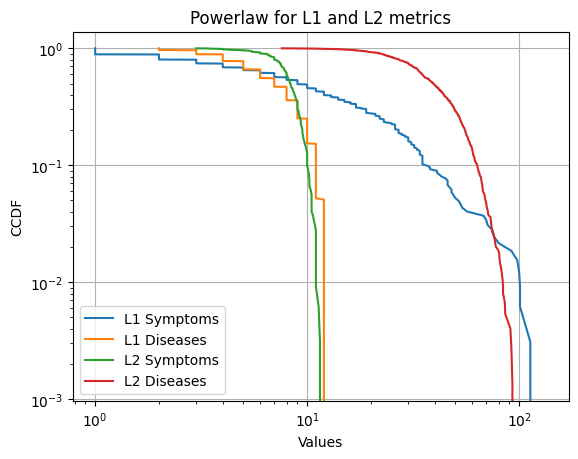
\includegraphics[width=\columnwidth]{powerlaw_hid_metrics.png}
    \caption{Power Law Distribution of the level 1 and level 2 metrics}
    \label{fig:powerlaw_hid_metrics}
\end{figure}
\subsubsection*{Statistical Validation of SI and DI}

In our statistical validation of the Symptom Influence (\textit{SI}) and Disease Influence (\textit{DI}) indices at level-2,
we aimed to discern whether these higher-order metrics provide additional information compared to level-1,
and whether this information is statistically significant.
Our null hypothesis (\textbf{H0}) posited that level-2 metrics do not offer additional insights beyond level-1,
while the alternative hypothesis (\textbf{H1}) suggested the opposite.\\
Upon generating 5000 random networks with the same level-1 properties as the original network,
we calculated z-scores for both Symptom Influence (\textit{SI}) and Disease Influence (\textit{DI}) at level-2.\\
Remarkably, the z-score distribution (Figure~\ref{fig:pdf_z_score}) for both symptoms and diseases exhibited a shape quite similar to a Gaussian distribution,
with means close to zero.\\
For symptoms, the z-scores ranged between -4 and 3, indicating that the level-2 Symptom Influence (\textit{SI})
values were generally lower than the mean but still within a reasonable range. This suggests that, on average,
symptoms tend to exhibit a level-2 influence that aligns closely with the overall network structure.\\
Similarly, for diseases, the z-scores ranged from -3 to 4, signifying that the level-2 Disease Influence
(\textit{DI}) values were distributed around the mean.
This implies that diseases, on average, have a level-2 influence that aligns with the overall network structure,
showcasing a balance between localized effects and broader impacts.\\
The proximity of the mean to zero in both distributions suggests that, on average,
the level-2 metrics for both symptoms and diseases do not significantly deviate from the null model.
However, the broader range of z-scores signifies the presence of nodes with both positive and negative deviations,
underscoring the heterogeneous nature of influences within the symptom-disease network.\\
In conclusion, our statistical validation reinforces that while the level-2 metrics follow a distribution akin to a Gaussian,
the nuanced deviations reflected by the z-scores
for both symptoms and diseases underscore the diverse and context-dependent nature of their influences within the intricate network structure.

\begin{figure}[H]
    \centering
    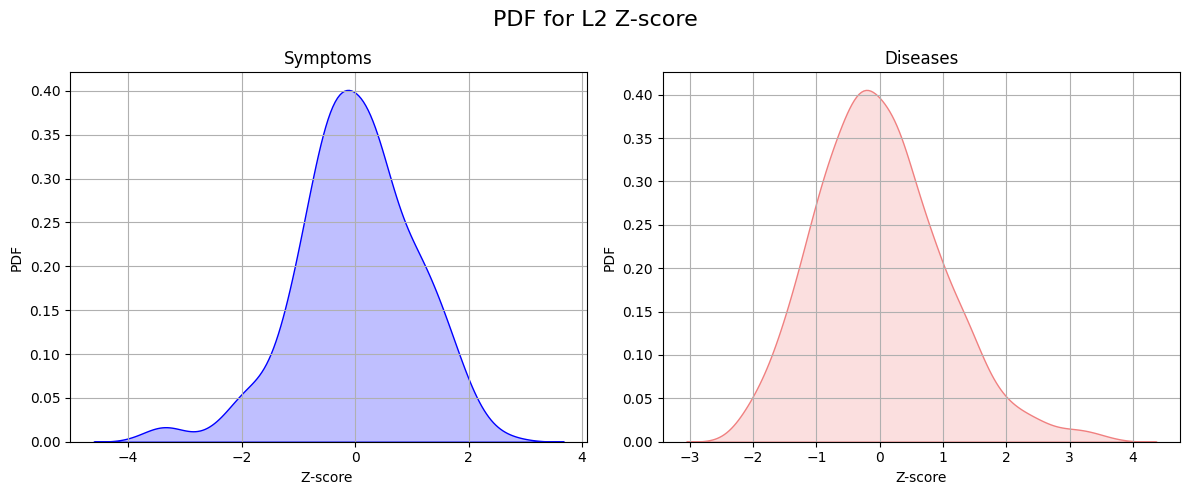
\includegraphics[width=\columnwidth]{PDF_z_score.png}
    \caption{Probability Density Function of the z-scores}
    \label{fig:pdf_z_score}
\end{figure}
% END: degree distribution and power law

\subsection{Betweenness Centrality}
% BEGIN: betweenness centrality
The examination of betweenness centrality in our bipartite network, as depicted in Figure~\ref{fig:bet_all},
reveals a Power Law Distribution, indicative of a scale-free structure. This implies the presence of a few central
nodes that act as pivotal connectors, while the majority of nodes exhibit lower betweenness centrality.

\begin{figure}[H]
    \centering
    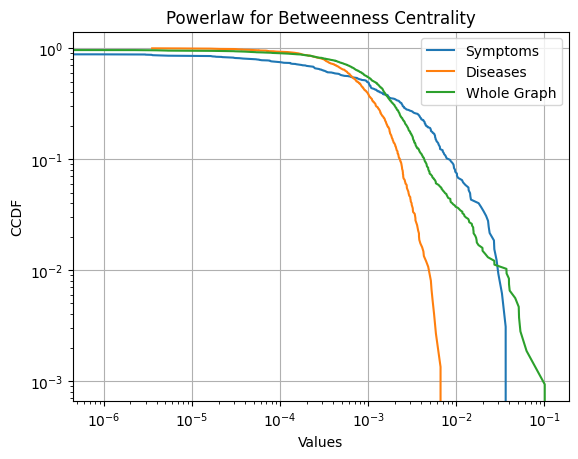
\includegraphics[width=\columnwidth]{bet_all.png}
    \caption{Betweenness Centrality CDFs}
    \label{fig:bet_all}
\end{figure}
\noindent
Upon dissecting the centrality values into symptoms and diseases (see Figures~\ref{fig:bet_diseases} and~\ref{fig:bet_symptoms}),
a notable observation emerges: symptoms tend to have higher betweenness centrality compared to diseases. To decipher the
significance of this result, it's essential to delve into the interpretation of betweenness centrality.

\begin{figure}[H]
    \centering
    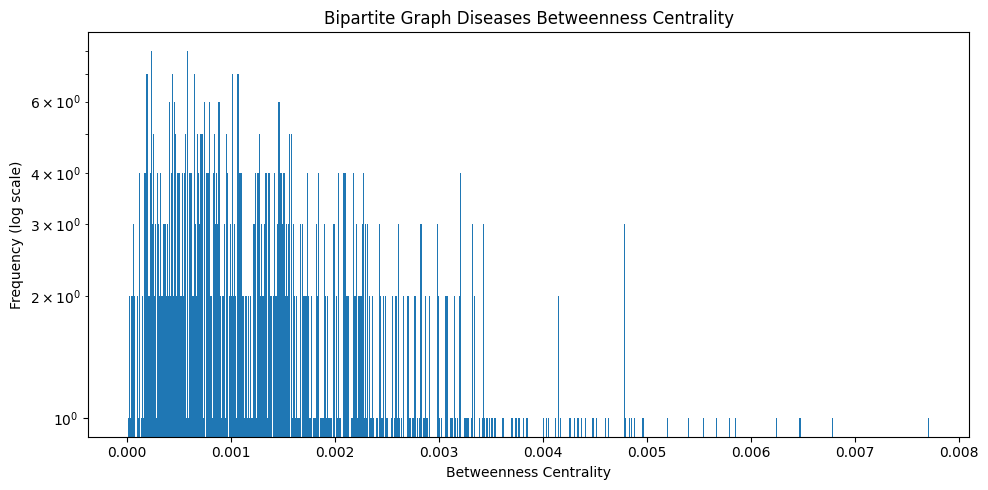
\includegraphics[width=\columnwidth]{bet_diseases.png}
    \caption{Betweenness Centrality of the diseases}
    \label{fig:bet_diseases}
\end{figure}
\noindent
\begin{figure}[H]
    \centering
    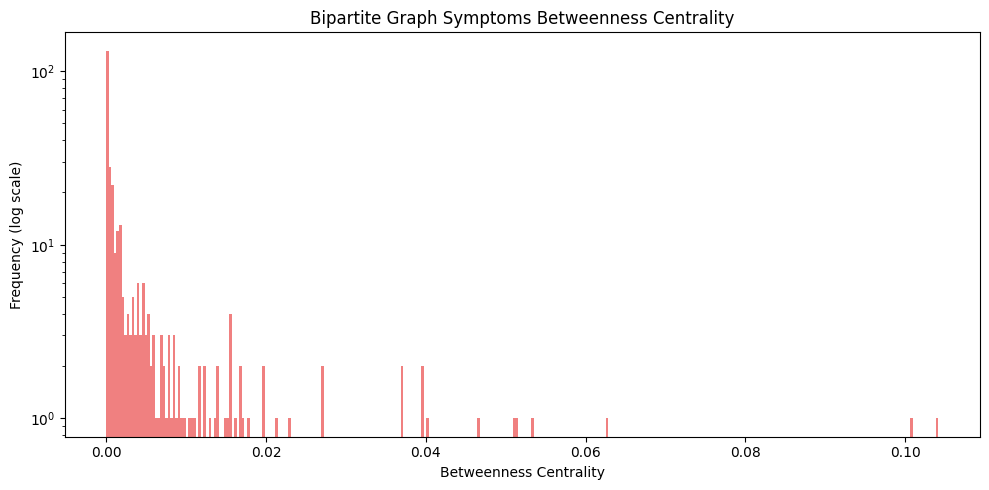
\includegraphics[width=\columnwidth]{bet_symptoms.png}
    \caption{Betweenness Centrality of the symptoms}
    \label{fig:bet_symptoms}
\end{figure}
\noindent
In general, a symptom exhibits high betweenness centrality when it is linked to numerous diseases, and these diseases,
in turn, are connected to a relatively limited set of symptoms. Conversely, a disease attains high betweenness centrality
when it connects to numerous symptoms, and these symptoms are associated with relatively few diseases.\\
Analyzing our results (L1 and L2), it becomes evident that the higher betweenness centrality of symptoms is attributed
to their connections with a multitude of diseases, while diseases, on the contrary, are linked to a relatively limited
number of symptoms. From a predictive standpoint, this outcome presents a challenge as each symptom is not sufficiently
specific, contributing to a broad array of disease classes.\\
Figure~\ref{fig:bet_top} highlights the top 10 nodes with the highest betweenness centrality, all of which are symptoms.
As anticipated, these symptoms are more generic in nature, aligning with their central role in connecting various diseases.

\begin{figure}[H]
    \centering
    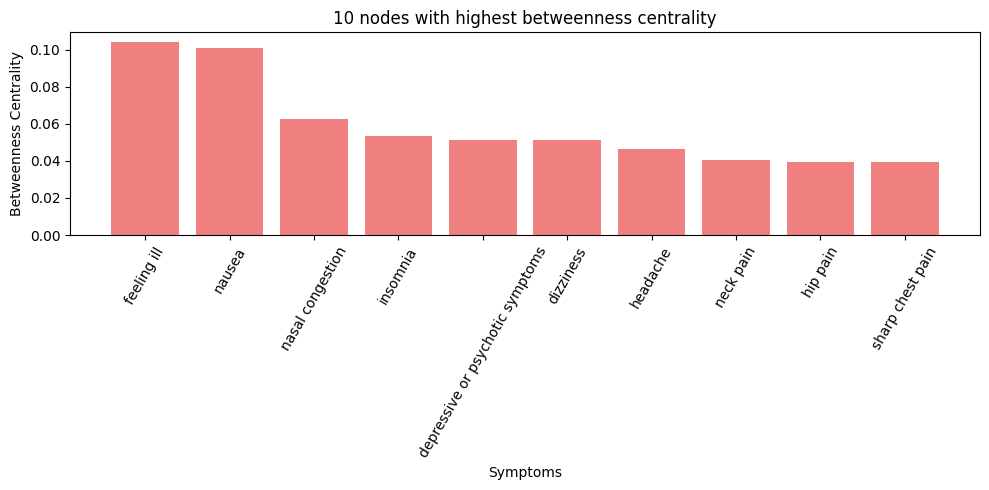
\includegraphics[width=\columnwidth]{bet_top.png}
    \caption{Top 10 nodes with the highest betweenness centrality}
    \label{fig:bet_top}
\end{figure}
\noindent
% END: betweenness centrality

\subsection{Communities}

% BEGIN: communities
The identification of communities within the network serves a dual purpose – facilitating network interpretation
and enhancing the capabilities of our ML prediction model.\\
From a network interpretation perspective, communities offer insights into disease-symptom relationships.
A community of symptoms signifies a set of symptoms that frequently co-occur within the same diseases, while a
community of diseases identifies a set of diseases often co-occurring within the same symptoms. The sizes of
different communities are illustrated in Figure~\ref{fig:com_sizes_all}.

\begin{figure}[H]
    \centering
    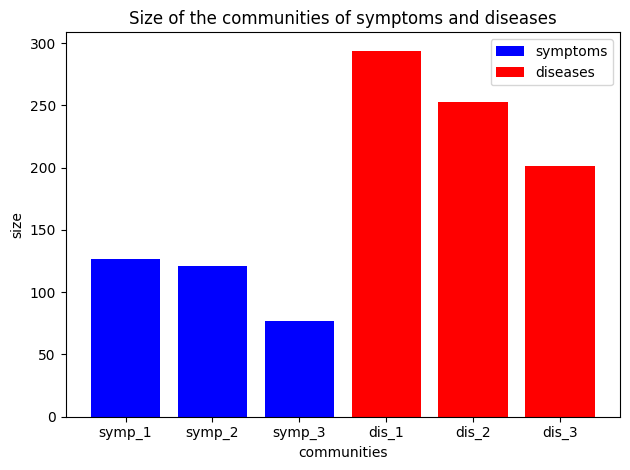
\includegraphics[width=\columnwidth]{com_sizes_all.png}
    \caption{Sizes of the communities of symptoms and diseases}
    \label{fig:com_sizes_all}
\end{figure}
\noindent
For clinical relevance, examining symptoms communities provides valuable information about diseases associated
with these symptoms. This is exemplified in Figures~\ref{fig:com1_symptoms},~\ref{fig:com2_symptoms},
and~\ref{fig:com3_symptoms}. As an illustration, in the community 1 of symptoms (Figure~\ref{fig:com1_symptoms}),
`herniated disk' is the third most pointed disease by the symptoms of the community, with each symptom pointing,
on average, to three diseases.

\begin{figure}[H]
    \centering
    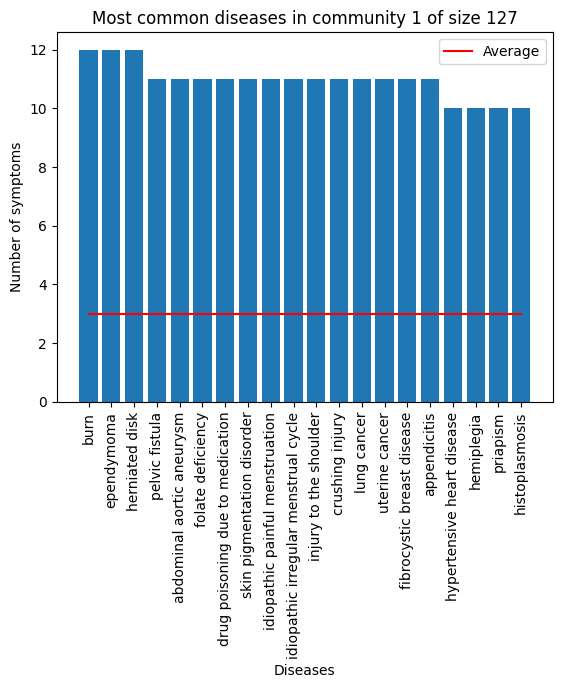
\includegraphics[width=\columnwidth]{com1_symptoms.png}
    \caption{Community 1 of symptoms}
    \label{fig:com1_symptoms}
\end{figure}
\noindent
A similar study can be conducted for communities of diseases, as depicted in Figures~\ref{fig:com1_diseases},
~\ref{fig:com2_diseases},~\ref{fig:com3_diseases}. This information aids in profiling diseases and understanding
the significance of each symptom. For instance, in community 1 of diseases (Figure~\ref{fig:com1_diseases}),
the symptom `sharp abdominal pain' is present in almost half of the diseases in the community, indicating its
generic nature and limited discriminatory value.

\begin{figure}[H]
    \centering
    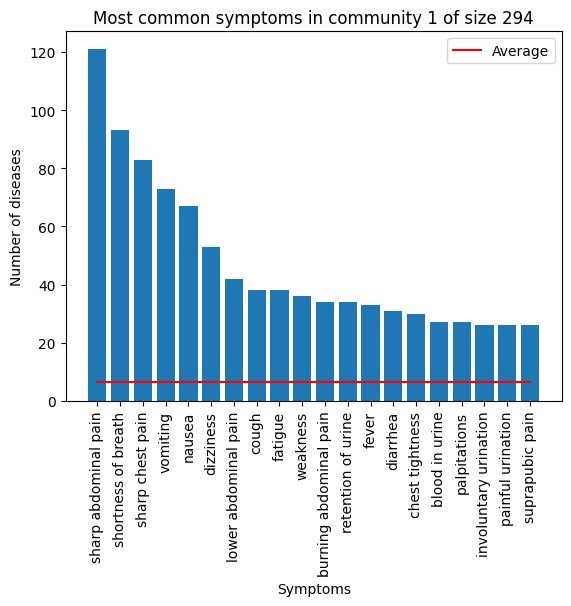
\includegraphics[width=\columnwidth]{com1_diseases.png}
    \caption{Community 1 of diseases}
    \label{fig:com1_diseases}
\end{figure}
\noindent
Transitioning to the creation of features for the ML model, two types of features were developed:\\

\begin{itemize}
    \setlength\itemsep{1em} % set space between items

    \item \textbf{Community Count:} This feature counts how many symptoms of the symptom vector belong to each community.
          Each symptom community is characterized by different pointed diseases. The model can learn to prioritize
          diseases associated with the community with the highest count.

    \item \textbf{Community Size:} This feature replaces each symptom in the symptom vector with the size of the
          community to which the symptom belongs. It enables the model to distinguish between symptoms belonging to small and
          large communities, injecting community information into the model beyond basic one-hot encoding of symptoms.
\end{itemize}
\noindent
It is noteworthy that communities can also contribute to improving the computational efficiency of the model.
For example, a symptom associated with many diseases may be less informative and could potentially be removed from the
symptom vector. However, we opted for a comprehensive approach using a combination of L1 and L2 measures to address this issue.

% END: communities

\subsection{Most Important Actors}
\label{subsec:most_important_actors}
% BEGIN: most important symptoms/diseases (4 classes)

As previously mentioned, our objective extends beyond feature extraction; we aim to leverage network information to
enhance the computational efficiency of the model. The strategy involves reducing the number of symptoms,
retaining only the most significant ones, to decrease training time while maintaining high accuracy.
Various approaches were tested, including L1, L2, betweenness centrality, and the degree of the unipartite projection
of symptoms. To select the most appropriate approach, we examined the correlation between these features
(Figure~\ref{fig:feat_corr}). Indeed, a high correlation between features means that they provide
similar information, and therefore retaining both features would be redundant. On the other hand,
a low correlation between features indicates that they provide complementary information, and this enhances
in a considerable way the quality of the choice.\\
For this reason, as clearly shown in Figure~\ref{fig:feat_corr}, we decided to use L1 and L2 to discriminate
among the symptoms in a more effective manner.

\begin{figure*}[!t]
    \centering
    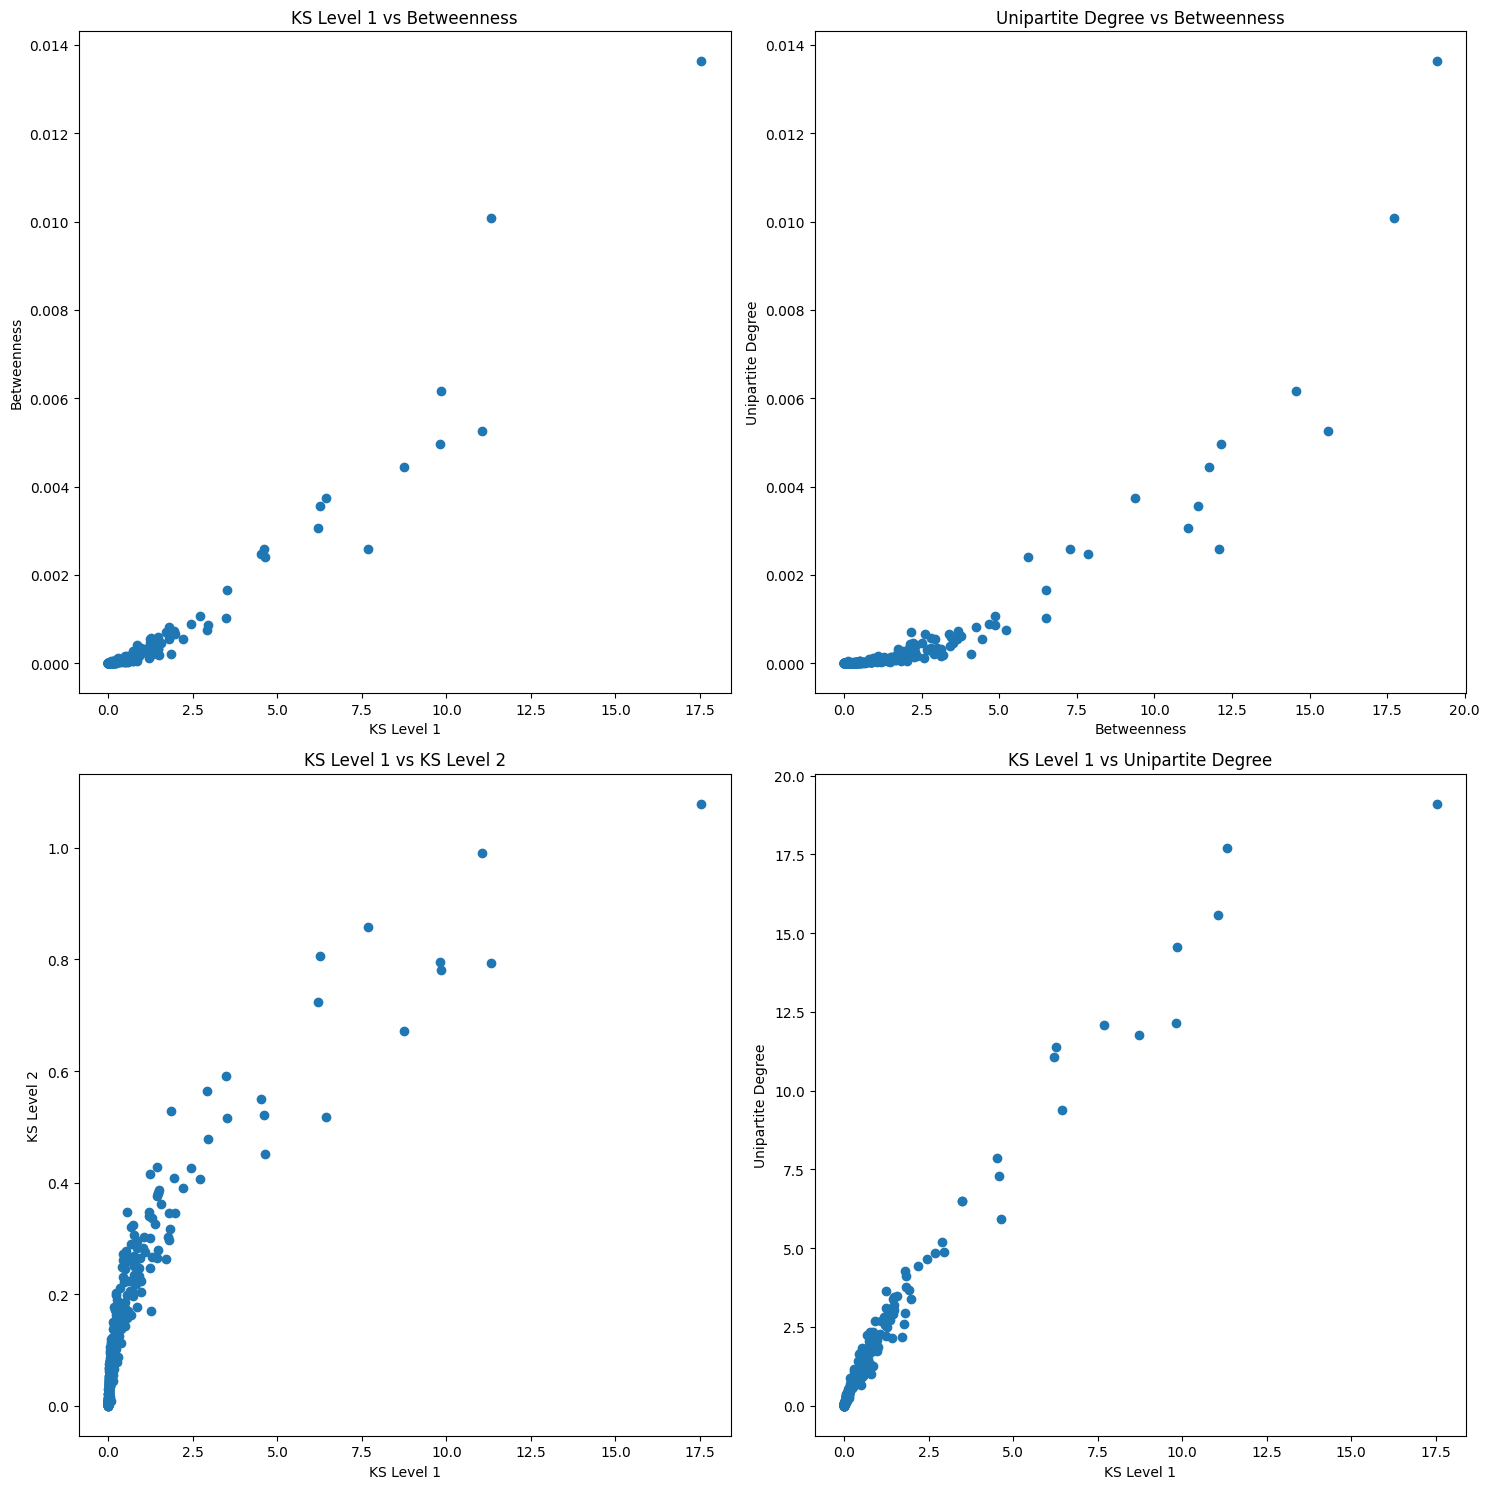
\includegraphics[width=\textwidth]{feat_corr.png}
    \caption{Correlation between features}
    \label{fig:feat_corr}
\end{figure*}

To practically create the classes, we need to define thresholds for L1 and L2. We decided to consider
a symptom as very important for our model if it is present in less than 0.5 times the average of L1 diseases,
translating into a threshold of 8.21 for L1. Consequently, we adjusted the L2 threshold to maintain a proper balance
between the classes, setting it to 8.

\begin{figure}[H]
    \centering
    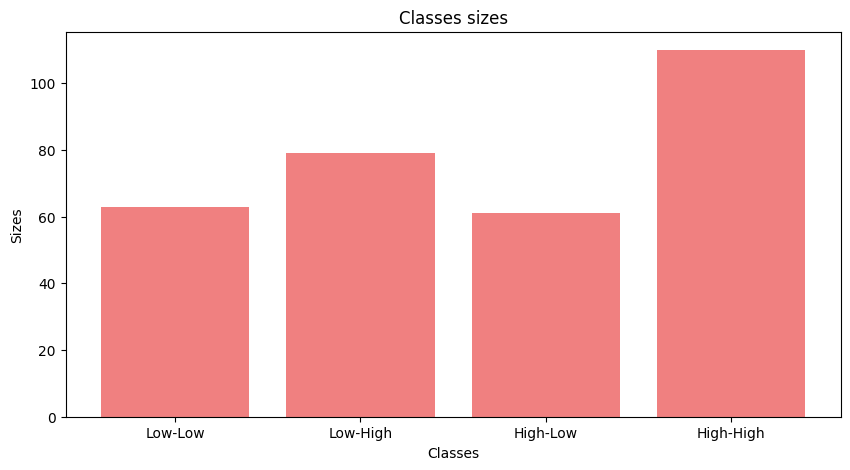
\includegraphics[width=\columnwidth]{symptoms_classes.png}
    \caption{Symptoms divided into the four classes}
    \label{fig:symptoms_classes}
\end{figure}

\begin{figure}[H]
    \centering
    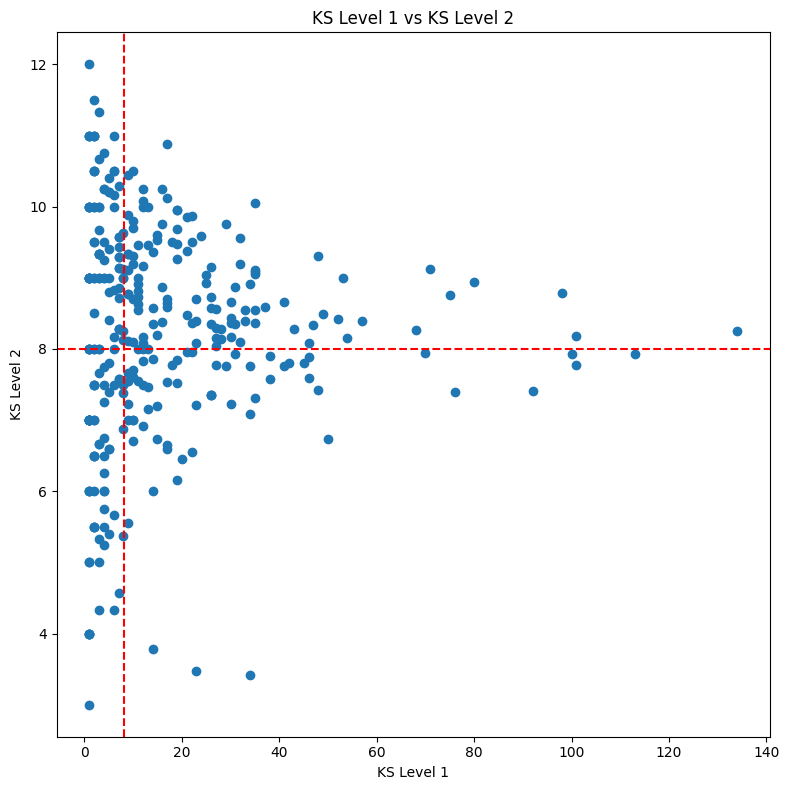
\includegraphics[width=\columnwidth]{l1_l2_division.png}
    \caption{Division based on L1 and L2 values}
    \label{fig:l1_l2_division}
\end{figure}
\noindent
<<<<<<< HEAD
While the analytical approach relying on correlation analysis lays a robust foundation for feature selection,
it is equally crucial to invest effort in interpreting the results. This interpretive step facilitates a
more profound understanding of the solution.\\
=======


\noindent
As demonstrated in Figure~\ref{fig:symptoms_classes}, the four classes have different sizes, and more importantly,
they provide very different and valuable information.

>>>>>>> cfd6877f42935cc11cb2837ca974703eda0c385f
To shed light on these classes, a brief reminder of the meanings of L1 and L2 is warranted. L1 denotes the number
of diseases associated with a symptom, whereas L2 quantifies the number of symptoms linked to those diseases.
As a result, we categorize the features into the following classes:\\

\begin{itemize}
    \setlength\itemsep{1em}
    \item \textbf{High L1 - High L2}: Symptoms with high degree and high L2. These symptoms are less crucial for
          prediction as they contribute to many classes (diseases), which are also connected to many other symptoms.
    \item \textbf{High L1 - Low L2}: Symptoms with high degree and low L2. These symptoms should not be removed a
          priori since they can be useful. For instance, a symptom may be associated with many diseases, but those
          diseases may only be associated with that symptom. In this case, the symptom is very important for prediction.
    \item \textbf{Low L1 - High L2}: Symptoms with low degree and high L2. These symptoms may be important for
          prediction, as they contribute to few diseases.
    \item \textbf{Low L1 - Low L2}: Symptoms with low degree and low L2. These symptoms are the most important
          for prediction since they contribute to few classes (diseases), and those classes are also connected to
          few other symptoms.
\end{itemize}

\noindent
According to the above considerations, we can start from the last class and iteratively add symptoms from the
other classes, monitoring the impact on both accuracy and training time.
The results are analyzed in Section~\ref{sec:results_ML}.\\
<<<<<<< HEAD
To practically create the classes, we need to define thresholds for L1 and L2. We decided to consider
a symptom as very important for our model if it is present in less than 0.5 times the average of L1 diseases,
translating into a threshold of 8.21 for L1. Consequently, we adjusted the L2 threshold to maintain a proper balance
between the classes, setting it to 8.\\
=======

>>>>>>> cfd6877f42935cc11cb2837ca974703eda0c385f
Figures~\ref{fig:symptoms_classes} and~\ref{fig:l1_l2_division} illustrate the division of symptoms into the four classes.
The same entire analysis was conducted for diseases, in this case focusing on the high-L1-high-L2 class, which contains
the most complex diseases under a symptomatology perspective. The results are reported in Figures~\ref{fig:diseases_classes}
and~\ref{fig:high_l1_high_l2_class}.\\


\noindent
To provide a complete picture of the most important symptoms we report the composition of the low-L1-low-L2 class
in Figure~\ref{fig:low_l1_low_l2_class}.\\

\begin{figure*}[!t]
    \centering
    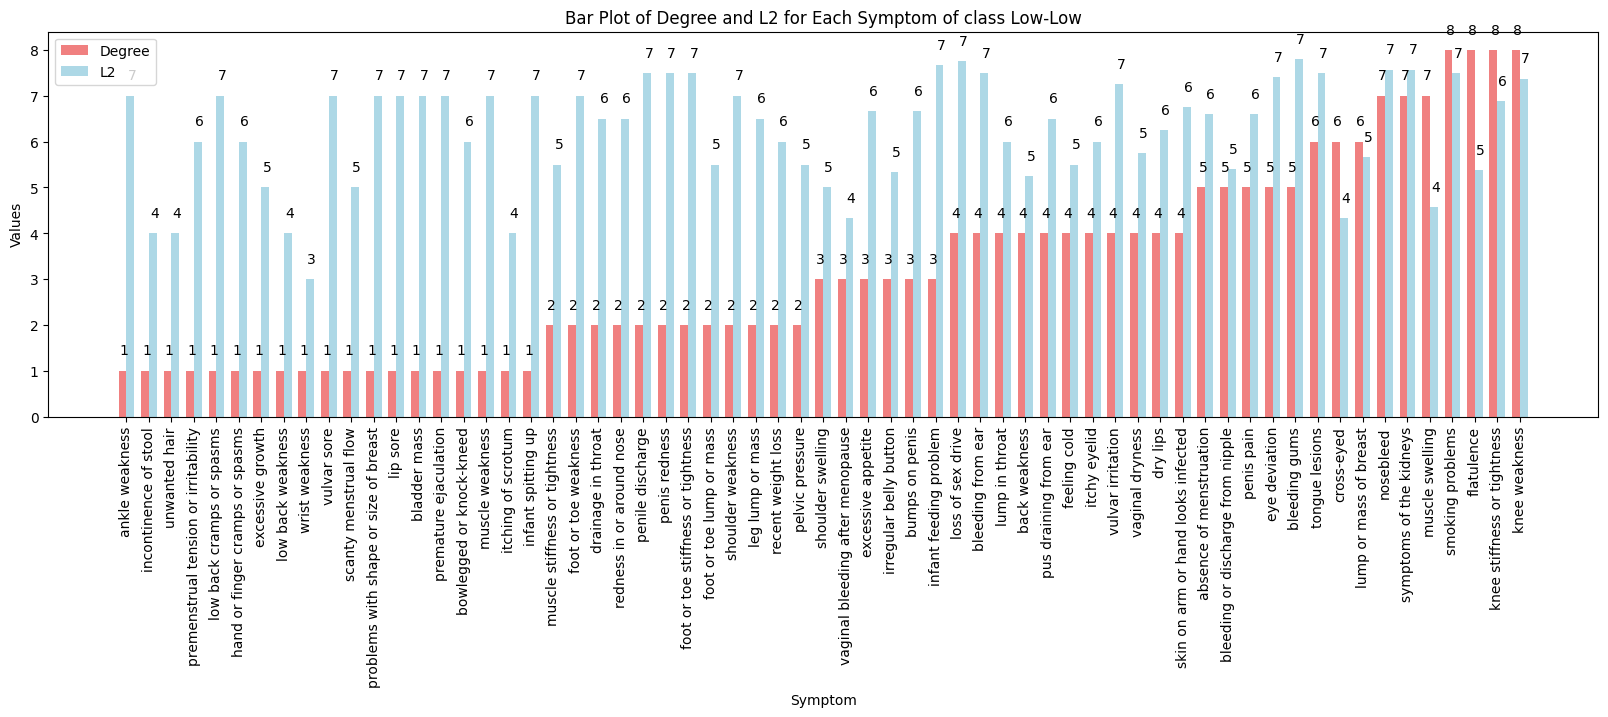
\includegraphics[width=\textwidth]{low_l1_low_l2_class.png}
    \caption{Composition of the low-L1-low-L2 class for symptoms}
    \label{fig:low_l1_low_l2_class}
\end{figure*}

% END: most important symptoms/diseases (4 classes)





